%
\chapter{Materiais e Softwares Utilizados} \label{MateSof}

Este capítulo apresenta uma breve descrição dos principais materiais e softwares necessários para implementação dos projetos propostos.  

\section{Arduino}

Arduino~\footnote{https://www.arduino.cc/en/Guide/Introduction} é uma plataforma de prototipagem de código aberto baseada na fácil utilização do software e hardware. As placas Arduino são capazes de efetuarem leitura de uma entrada (sensores) e transformar em uma de saída (Atuadores). O projeto Arduino nasceu no Ivrea Interaction Design Institute como uma ferramenta fácil para prototipagem rápida, destinado a estudantes sem conhecimento aprofundado em eletrônica e programação. 

A plataforma Arduino possui uma IDE para a programação e para gravar códigos na placa, a IDE possui ainda suporte a Linux, Mac e Windows. 

Existem diversas placas de hardware Arduino, sendo a mais comum a Arduino Uno. As placas diferem basicamente no microcontrolador embutido, no número de entradas/saídas, na frequência de processamento e entre outras configurações.

Neste Material vamos utilizar o Arduino Uno por ser facilmente encontrado no mercado e apresentar baixo custo de aquisição se comparado com outras plataformas de hardware.

A conexão de novos componentes no Arduino é possível por meio de placas de expansão (\textit{shields}), essa placas aumentam as funcionalidades do Arduino. Os \textit{shields} mais conhecidos são os \textit{shields} para controle de motores~\footnote{https://www.arduino.cc/en/Main/ArduinoMotorShieldR3} e o Ethernet para comunicação do Arduino com a Internet, como o da Figura~\ref{fig:motorControl}.  

\begin{figure}[ht]
      \centering
      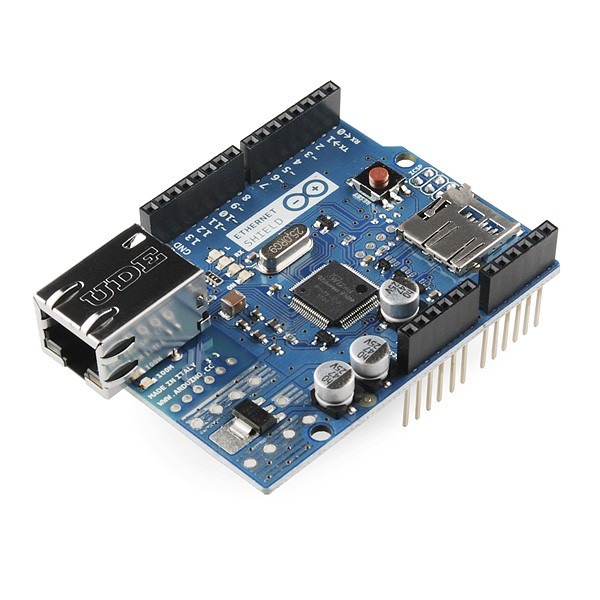
\includegraphics[scale=0.35]{figuras/image_321.jpg}
      \caption{Shield para controle de motores}
      \label{fig:motorControl}
\end{figure}

A comunicação do Arduino com \textit{shields} é realizada pelo protocolo Serial Peripheral Interface (SPI)~\footnote{https://www.arduino.cc/en/Reference/SPI
}  , ele é um protocolo de dados seriais síncronos utilizado em microcontroladores para comunicação entre o microcontrolador e um ou mais periféricos, sendo que também pode ser utilizado entre dois microcontroladores.

A comunicação SPI sempre tem um master. Isto é, sempre um será o master e o restante será slave. Por exemplo, o Arduino é o master e os outros periféricos são slaves. Esta comunicação contém 4 conexões:

\begin{itemize}
  \item MISO (Master IN Slave OUT) - Dados do Slave para Master;
  \item MOSI (Master OUT Slave IN) - Dados do Master para Slave;
  \item SCK (Serial Clock) - Clock de sincronização para transmissão de dados entre o Master e Slave;
  \item SS (Slave Select) - Seleciona qual Slave receberá os dados.
\end{itemize}

\subsection{Arduino IDE}

Para programação no arduino, utiliza-se a linguagem Wiring. O ambiente de programação oferece recursos que facilitam a criação de aplicações e sua gravação no dispositivo.

Os projetos (Sketches) são escritos na linguagem Wiring e salvos com a extensão .ino, possuindo a seguinte estrutura:

\lstinputlisting[language=C++, caption={Estrutura código Arduino}]{code/arduino.ino}

A função setup() é o código de inicialização dos componentes, enquanto a função loop é o laço principal do programa, que contém o código que será executado repetidamente.

\subsection{Arduino Uno}

O Arduino Uno~\footnote{https://www.arduino.cc/en/Main/ArduinoBoardUno} opera com uma velocidade de clock de 16 MHz, possui 14 pinos de entrada e saída digitais e 6 pinos de entrada e saída analógica, memória flash de 32 KB (0.5 KB usados pelo Bootloader), memória SRAM de 2 KB e 1 KB de memória EEPROM. 

A placa pode ser alimentada pela conexão USB ou por uma fonte de alimentação externa. Para alimentação externa é utilizado um conector Jack com positivo no centro, sendo que a placa suporta alimentação de 6 à 20 volts. Porém, é recomendado que a fonte de alimentação externa possua tensão entre 7 e 12 volts. 

A Figura~\ref{fig:arduino} ilustra o Arduino Uno utilizado neste projeto, ele tem 14 pinos de entradas/saídas digitais. Alguns desses pinos possuem funções especificas como PWM (pinos 3, 5, 6, 9, 10 e 11 ), comunicação serial (pinos 0 e 1) e interrupção externa (pinos 2 e 3).
Para interface com o mundo analógico, a placa Arduino UNO possui 6 entradas, onde cada uma tem a resolução de 10 bits.

\begin{figure}[ht]
      \centering
      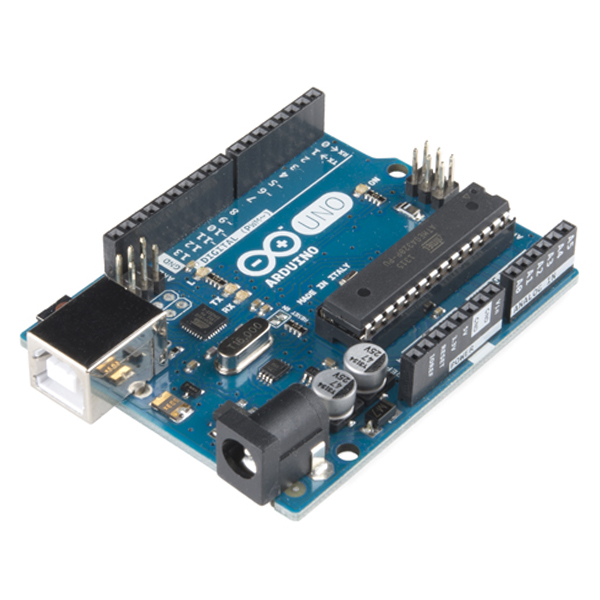
\includegraphics[scale=0.35]{figuras/arduino.jpg}
      \caption{Arduino Uno}
      \label{fig:arduino}
\end{figure}



\section{Radio RF - nRF24l01}

Nesta apostila vamos utilizar o módulo de rádio frequência nRF24l01~\footnote{http://www.nordicsemi.com/eng/Products/2.4GHz-RF/nRF24L01} fabricado pela Nordic, este módulo trabalha na frequência de 2.4 GHz.

A conexão é realizada por um conector de 8 pinos muito próximos uns dos outros, o que impossibilita a conexão direta do módulo com a protoboard. Sendo assim, a conexão com o módulo pode ser feita com jumpers macho-fêmea. Outra possibilidade é construir um shield para adaptação, para que o nRF24l01 encaixe na protoboard.

O alcance do módulo varia de 10 metros em ambiente fechado à 50 metros em ambiente aberto. Uma outra vantagem é que um mesmo módulo pode atuar como emissor ou receptor, apenas realizando-se uma configuração por software. Sua tensão de alimentação é de 1,9 à 3.6V, e os pinos de sinal podem trabalhar normalmente com nível de sinal de 5V. 

Existe uma versão do módulo com antena externa, essa versão possibilita distância maior de comunicação entre os módulos, porém tem preço maior e não é tão compacto quanto o módulo com antena embutida. 

\begin{figure}[ht]
      \centering
      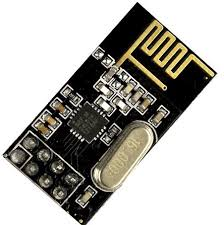
\includegraphics[scale=0.30]{figuras/nrf24l01.jpg}
      \caption{Rádio nRF24L01}
      \label{fig:nRF24L01}
\end{figure}



\section{Sensores e Atuadores}

Esta seção é uma breve descrição dos principais sensores e atuadores utilizados para realizar os projetos propostos nesse material.  

\subsection{DTH11}

O DTH11~\footnote{https://learn.adafruit.com/dht} é um sensor de baixo custo para a medição de temperatura e umidade do ambiente. Sua faixa de medição de temperatura vai de 0° a 50° Celsius, com 2\% de margem de erro. Já a medição de umidade pode variar de 20\% até 90\% com precisão de 5\%.

O sensor possui 4 pinos: um pino para o GND(ground), um para a alimentação(5V), um pino para envio dos dados que é conectado a uma entrada digital do Arduino e um pino que não é utilizado.

\begin{figure}[ht]
      \centering
      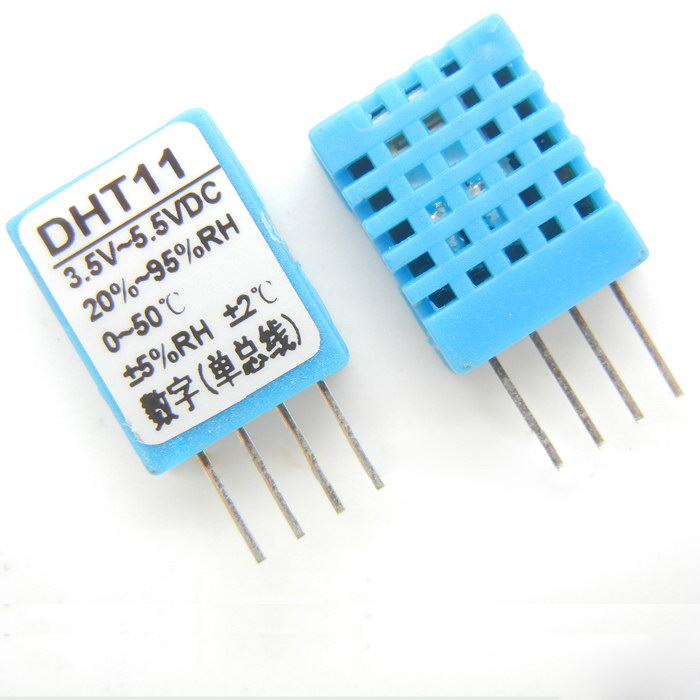
\includegraphics[scale=0.20]{figuras/FDHT11.jpg}
      \caption{Sensor DTH11}
      \label{fig:Sdth11}
\end{figure}

\subsection{LDR}

O LDR (do inglês, Light Dependent Resistor), ou Resistor dependente de Luz, é uma fotorresistência, ou seja, um resistor cuja resistência varia de acordo com a intensidade da luz que incidir sobre ele. 

Utilizando um multímetro pode-se medir a resistência de um LDR quando exposto a uma determinada intensidade de luz. Basicamente, um LDR vai ter sua resistência máxima quando estiver em completa escuridão e mínima quando uma luz muito brilhante estiver incindindo sobre ele.

\begin{figure}[H]
      \centering
      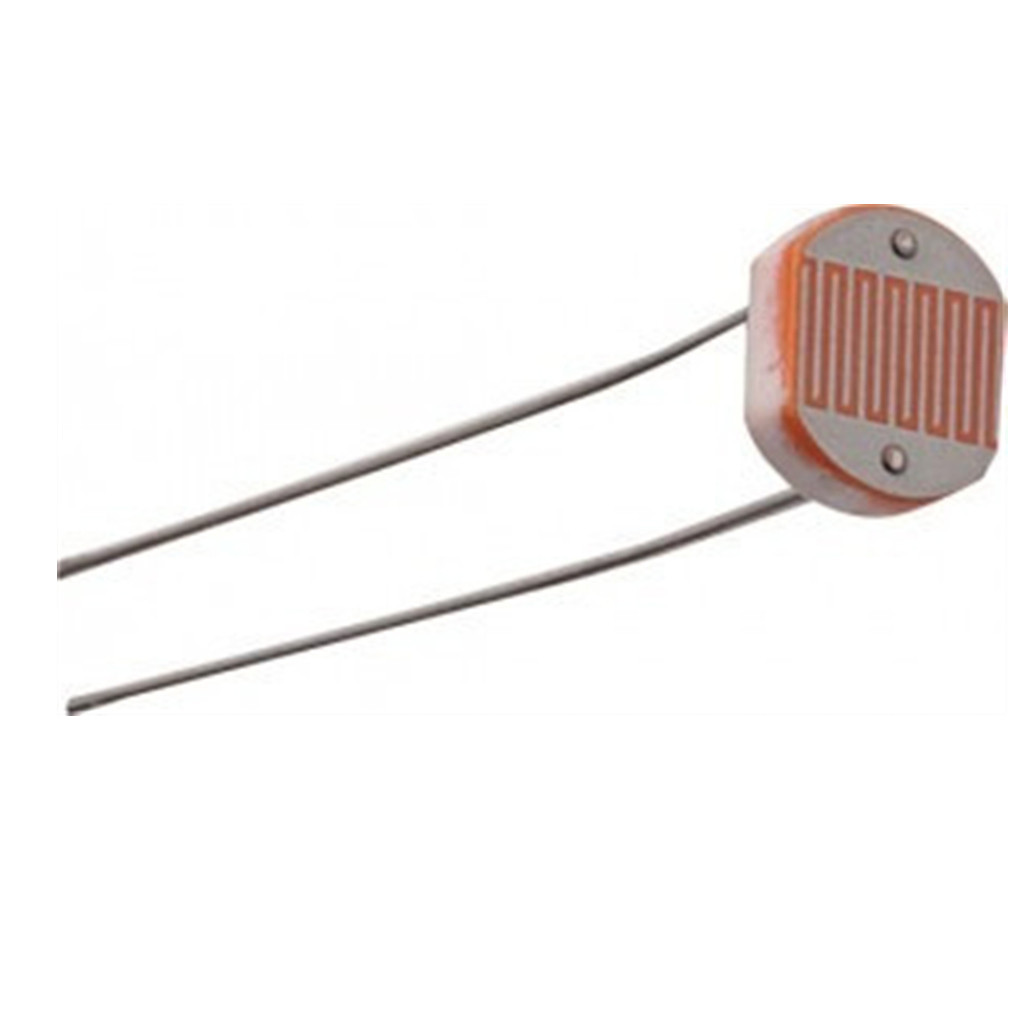
\includegraphics[scale=0.10]{figuras/Fldr.jpg}
      \caption{Sensor LDR}
      \label{fig:SLDR}
\end{figure}



%[https://en.wikipedia.org/wiki/Photoresistor]

\subsection{Relé}

O relé é um dispositivo eletromecânico capaz de desligar ou ligar outros dispositivos. Basicamente, o relé é acionado quando uma corrente elétrica passa a percorrer as espiras da bobina do mesmo, criando assim um campo magnético que atrai ou repele uma alavanca responsável por ativar ou desligar o outro componente ligado ao relé. 

\begin{figure}[ht]
      \centering
      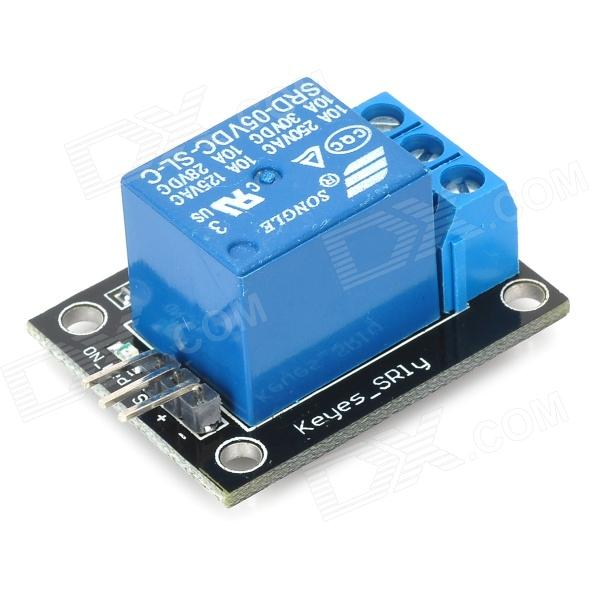
\includegraphics[scale=0.25]{figuras/Frele.jpg}
      \caption{Atuador relé}
      \label{fig:Arele}
\end{figure}

% incluir exemplo de uso

\subsection{Sensor de Movimento (PIR)}

O sensor de movimento (PIR)~\footnote{https://learn.adafruit.com/pir-passive-infrared-proximity-motion-sensor/}é, basicamente, feito de um material piroelétrico, ou seja, seu potencial elétrico varia de acordo com a temperatura, tornando-o capaz de detectar alguns níveis de radiação infravermelha. Ele é construído em duas metades e as duas são conectadas de forma que a diferença de potencial entre elas seja interpretada como um nível alto ou baixo, fazendo assim a detecção de movimento.

\begin{figure}[ht]
      \centering
      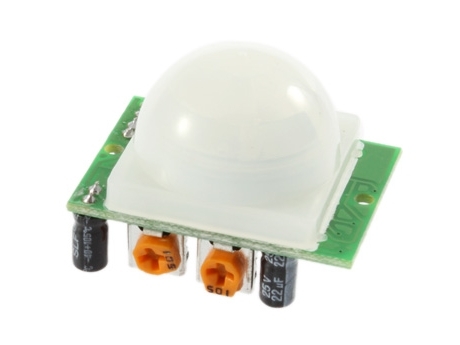
\includegraphics[scale=1.20]{figuras/Fpir.png}
      \caption{Sensor de Movimento PIR}
      \label{fig:SPIR}
\end{figure}

% explicar porque funciona p/ detectar movimento


\subsection{LED}

Light Emitting Diode (LED) ou diodo emissor de luz, é utilizado para emissão de luz em locais onde lâmpadas não são viáveis, por exemplo em produtos da microeletrônica, como sinais de avisos. Existem também LEDs de tamanhos maiores, como os utilizados em sinais de trânsito.

Uma característica marcante do LED diz respeito ao seu baixo consumo de energia, sendo uma alternativa viável para iluminação de ambientes. Outra característica importante é que sua durabilidade é maior que as outras formas de emissão de luz presentes no mercado.

Na maioria dos projetos vamos utilizar o LED como atuador para emitir sinais de aviso. Mais detalhes sobre o funcionamento do LED estão disponíveis em http:\/\/electronics.howstuffworks.com\/led.htm

% [https://en.wikipedia.org/wiki/Light-emitting_diode]
% [http://electronics.howstuffworks.com/led.htm]

\begin{figure}[ht]
      \centering
      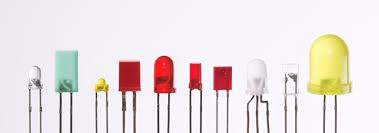
\includegraphics[scale=0.50]{figuras/Fled.jpg}
      \caption{LEDs}
      \label{fig:Aled}
\end{figure}


\section{Protoboard}

A Protoboard é uma placa com uma matriz de furos e conexões condutoras utilizadas para a prototipação de circuitos eletrônicos.

\begin{figure}[ht]
      \centering
      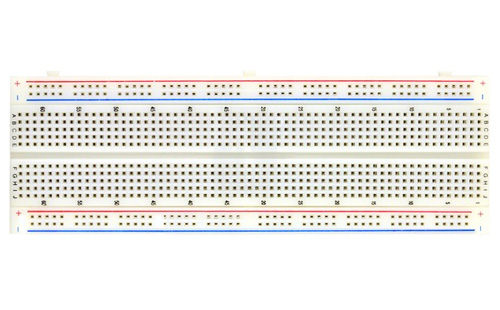
\includegraphics[scale=0.50]{figuras/FProtoboard_2_M.jpg}
      \caption{Protoboard}
      \label{fig:protoboard}
\end{figure}

A Figura~\ref{fig:protoboard} ilustra uma protoboard. Essa placa tipicamente possui trilhas conectadas na vertical que possibilitam a ligação entre componentes e trilhas isoladas na horizontal. 

\section{Conexão de todas as partes}

Para conectar os sensores e atuadores à placa do Arduino, é utilizado cabo jumper. Pode ser encontrado em 3 combinações: macho-macho, macho-fêmea e fêmea-fêmea.

A Figura~\ref{fig:Jmacho} representa jumpers macho. 

\begin{figure}[H]
      \centering
      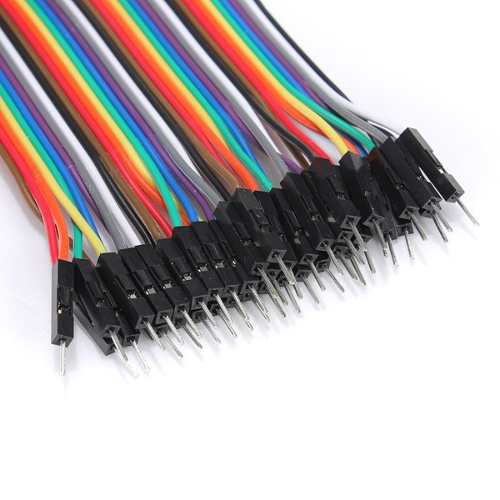
\includegraphics[scale=0.25]{figuras/jumperMachoo.jpg}
      \caption{Jumper Macho}
      \label{fig:Jmacho}
\end{figure}

A Figura~\ref{fig:Jfemea} representa jumpers fêmea.

\begin{figure}[H]
      \centering
      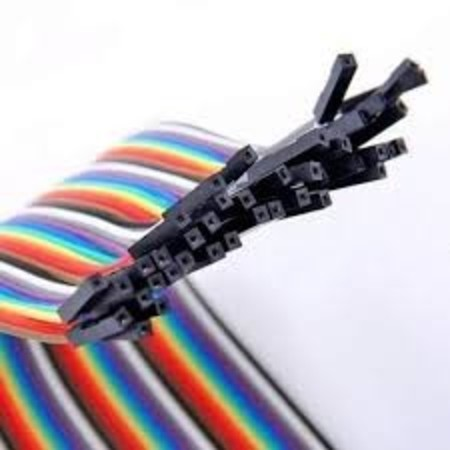
\includegraphics[scale=0.30]{figuras/Jfemea.jpg}
      \caption{Jumper Fêmea}
      \label{fig:Jfemea}
\end{figure}

%explicar/foto macho-macho, macho-femea e femea-femea

\section{Conectando o Arduino ao Rádio}

O rádio nRF24l01+ se comunica com Arduino via interface SPI. O rádio deve ser alimentado com uma tensão de 3.3 volts. 

Como o rádio possui conector de 8 pinos, não é possível conectá-lo a protoboard. Então, devemos utilizar conectores macho-fêmea, como ilustra a Figura~\ref{fig:gat}, para fazer ligação ou construir um shield para adaptação do módulo.

\begin{figure}[H]
      \centering
      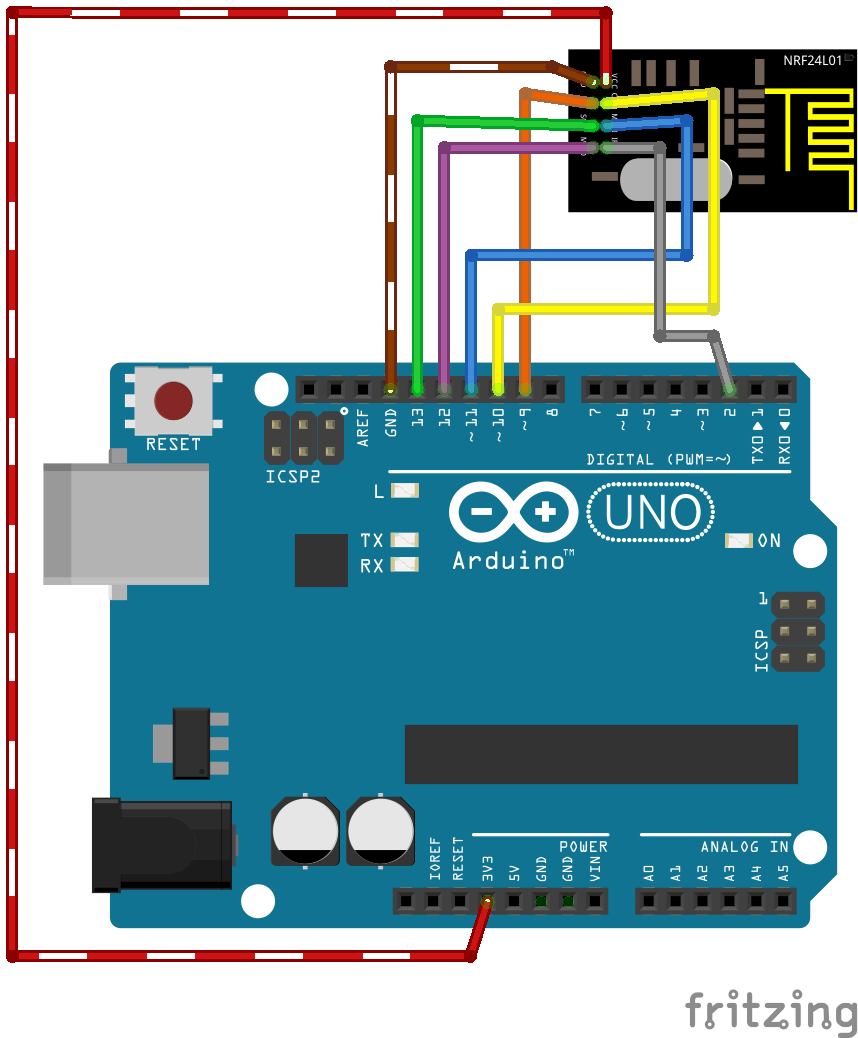
\includegraphics[scale=0.50]{figuras/gateway.png}
      \caption{Conexão rádio e Arduino Uno}
      \label{fig:gat}
\end{figure}

\section{Biblioteca Mysensors}

Mysensors~\footnote{http://www.mysensors.org/} é uma API que fornece um conjunto de protocolos e rotinas para comunicação entre o Arduino, o Rádio transmissor e sensores. 
Com esta biblioteca é possível criar uma abstração de algumas camadas de hardware e software evitando que o usuário tenha que implementar rotinas de baixo nível e protocolos para realizar a comunicação entre o Arduino e Módulo de rádio frequência. A biblioteca fornece códigos de exemplos e uma estrutura de rede já implementada para Internet das Coisas. 

\subsection{Aplicações da biblioteca MySensors}

A biblioteca MySensors fornece uma infinidade de projetos com exemplos de sensores e atuadores já implementados. Algumas possibilidades de aplicação da biblioteca são:

\begin{itemize}
    \item Pequenas automações residenciais, tais como um portão de garagem automático que abre quando um carro se aproxima da entrada ou quando ativado pelo seu \textit{smartphone}; 

    \item Coletar a umidade do ambiente dentro da casa para controlar a ventilação;

    \item Criar uma fechadura inteligente para um determinado cômodo ou armário; 
    
    \item Criar um dispositivo que avisa através de uma mensagem em seu \textit{smartphone} quando a temperatura do frezzer subir caso alguém tenha deixado a porta aberta;

    \item Criar uma identificação única para seu cachorro para que somente ele possa entrar em sua casa.
\end{itemize}

\subsection{Instalar Mysensors}

MySensors é uma biblioteca que funciona integrada com a API do Arduino, para instalação basta adicioná-la a pasta \textit{libraries} do Arduino IDE.




